\documentclass[11pt,oneside,chapters]{starlink}

%\newcommand{\polpack}{\xref{\textsc{POLPACK}}{sun223}{}}

\usepackage{amsfonts}
\usepackage{longtable}
\usepackage{amsmath}
\usepackage{siunitx}

\stardoccategory {Starlink Cookbook}
\stardocinitials {SC}
\stardoccopyright{Copyright \copyright\ 2021 East Asian Observatory}
\stardocnumber   {22}
\stardoctitle    {The POL-2 Data Reduction Cookbook}
\stardocversion  {1.1}
\stardocabstract {
  This cookbook provides an introduction to POL-2 data reduction,
  using the Starlink facilities \smurf (the Sub-Millimetre
  User Reduction Facility) and in particular its command
  \xref{\task{pol2map}}{{sun258}{POL2MAP}}. This cookbook illustrates
  the various steps
  required to reduce the data, including an overview of the method. It
  also describes how to calibrate and display the data as images or
  vector maps.}

\stardocauthors{H.\ A.\ L.\ Parsons, D.\ S.\ Berry,
  M.\ G.\ Rawlings, and S.\ F.\ Graves}

\stardocdate{2021 July 15}

%-------------------------------------------------------------------

% Local Definitions
\newcommand{\xparam}[2]{\xref{#2}{sun258}{#1}}

%-------------------------------------------------------------------



\begin{document}
\scfrontmatter





% Acronyms section
\Acronyms

\begin{table}[h!]
\begin{tabular}{ll}
\textbf{CADC}   & Canadian Astronomy Data Centre\\
\textbf{FCF}    & Flux Conversion Factor\\
\textbf{FITS}   & Flexible Image Transport System\\
\textbf{GAIA}   & Graphical Astronomy and Image Analysis tool\\
\textbf{HWP}    & Half-Wave Plate\\
\textbf{ITC}    & Integration Time Calculator\\
\textbf{I}      & Total intensity \\
\textbf{IP}     & Instrumental Polarisation \\
\textbf{JCMT}   & James Clerk Maxwell Telescope\\
\textbf{NDF}    & Extensible N-Dimensional Data Format\\
\textbf{P}      & Percentage polarisation \\
\textbf{PCA}    & Principal Component Analysis \\
\textbf{I$_{p}$}     & Polarised intensity \\
\textbf{SCUBA-2}& Submillimetre Common User Bolometer Array-2\\
\textbf{SMURF}  & Sub-Millimetre User Reduction Facility\\
\textbf{SUN}    & Starlink User Note\\
\textbf{WCS}    & World Coordinate System\\
\end{tabular}
\end{table}


\newpage
\chapter{Introduction}
\label{sec:intro}

% set up page numbers in arabic numerals and restart from 1
\renewcommand{\thepage}{\arabic{page}}
\setcounter{page}{1}

\section{This cookbook}

This guide is designed to instruct POL-2 users on the best ways to
reduce and visualise their data using \starlink\ packages:
\smurf \cite{smurf}, \Kappa \cite{kappa}, polpack and \gaia \cite{gaia}.

This guide covers the following topics.
\begin{itemize}
\itemsep0em
\item \cref{Chapter}{sec:intro}{Chapter 1} -- Computer resources you'll need before getting started.
\item \cref{Chapter}{sec:pol2}{Chapter 2} -- A description of POL-2 and its observing modes.
\item \cref{Chapter}{sec:dr}{Chapter 3} -- POL-2 Data Reduction - The Theory
\item \cref{Chapter}{sec:rundr}{Chapter 4} -- POL-2 Data Reduction - Running pol2map
\item \cref{Chapter}{sec:display}{Chapter 5} -- POL-2 Image Display
\item \cref{Chapter}{sec:advanced}{Chapter 6} -- POL-2 Advanced Data Reduction 

\end{itemize}

Throughout this document, a percent sign (\texttt{\%}) is used to
represent the Unix shell prompt. What follows each \texttt{\%} will be
the text that should be typed by the user to initiate the described action.

\section{\xlabel{computing} Before you start: computing resources}
\label{sec:computing}

Unlike SCUBA-2 observations, POL-2 observations are far less memory intensive to reduce. 
Maps are down sampled to 2Hz within the reduction process. Assuming a typical 35 
minute POL-2 observation, the reduction requires 35 GB of memory (in comparison to SCUBA-2
maps that may require up to 96 GB of memory).

The main consideration for POL-2 reductions is processing power. PCA calculations in
makemap can be lengthy so a fast processors with lots of cores is advised.


\section{\xlabel{software}Before you start: software}

This manual uses software from the \starlink\ packages: \smurf\
\cite{smurf}, \Kappa\ \cite{kappa}, polpack and \gaia\ \cite{gaia}. 
Starlink software must be installed on your system, and Starlink 
aliases and environment variables must be defined before attempting 
to reduce any SCUBA-2 data.

\subsection{Data formats}
\label{sec:ndf}

Data files for POL-2 are the same as for SCUBA-2 and use 
the Starlink N-dimensional Data Format (NDF,
see Jenness et al.\ 2014\cite{ndf}), a hierarchical format which allows
additional data and metadata to be stored within a single file. \Kappa\
contains \xref{many commands}{sun95} {ap_classified}\ for examining and
manipulating NDF structures. The introductory sections of the \Kappa\
document (\xref{SUN/95}{sun95}{}) contain much useful information on
the contents of an NDF structure and how to manipulate them.

A single NDF structure describes a single data array with associated
meta-data. NDFs are usually stored within files of type ``\verb+.sdf+''.
In most cases (but not all), a single \verb+.sdf+ file will contain just
one top-level NDF structure, and the NDF can be referred to simply by
giving the name of the file (with or without the ``\verb+.sdf+'' prefix).
In many cases, a top-level NDF containing JCMT data will contain other
``extension'' NDFs buried inside them at a lower level. For instance, raw
files contain a number of NDF components which store observation-specific
data necessary for subsequent processing. The contents of these (and
other NDF) files may be listed with \HDSTRACEref. Each file holding raw
JCMT data on disk is also known as a `sub-scan'.

The main components of any NDF structure are:
\begin{itemize}
\item An array of numerical data (may have up to seven
dimensions---usually three for JCMT data);
\item An array of variance values corresponding to the numerical data
values;
\item An array holding up to eight boolean flags (known as ``quality
flags'') for each pixel;
\item World Coordinate System information;
\item History;
\item Data units
\item Other extensions items. These are defined by particular packages,
but usually include a list of FITS-like headers together with provenance
information that indicates how the NDF was created. Raw JCMT file also
include extensions that define the state of the telescope and instrument
at each time slice within the observation.
\end{itemize}

The \convert\ package contains commands \xref{\task{fits2ndf}}{sun55}{FITS2NDF} and
\xref{\task{ndf2fits}}{sun55}{NDF2FITS} that allow interchange between FITS
and NDF format.

\subsection{Initialising Starlink}
\label{sec:starinit}

The commands and environment variables needed to start up the required
Starlink packages (\smurf \cite{smurf}, \Kappa, \emph{etc.}) must first
be defined. For C shells (csh, tcsh), do:

\begin{terminalv}
% setenv STARLINK_DIR <path to the starlink installation>
% source $STARLINK_DIR/etc/login
% source $STARLINK_DIR/etc/cshrc
\end{terminalv}

before using any Starlink commands. For Bourne shells (sh, bash, zsh), do:

\begin{terminalv}
% export STARLINK_DIR=<path to the starlink installation>
% source $STARLINK_DIR/etc/profile
\end{terminalv}

\subsection{KAPPA and SMURF for data processing}
\label{sec:packinit}

The Sub-Millimetre User Reduction Facility, or \textsc{Smurf},
contains the Dynamic Iterative Map-Maker, which will process raw
SCUBA-2 data into images (see \smurfsun). \textsc{Kappa} meanwhile is
an application package comprising general-purpose commands mostly for
manipulating and visualising NDF data (see \kappasun). Before starting
any data reduction you will want to initiate both \textsc{Smurf} and
\textsc{Kappa}.

\begin{terminalv}
% smurf
% kappa
\end{terminalv}

After entering the above commands, you can access the help information
for either package by typing \texttt{smurfhelp} or
\texttt{kaphelp} respectively in a terminal, or by using the
\task{showme} facility to access the hypertext documentation. See
\cref{Section}{sec:help}{How to get help} for more information.



\begin{tip}
The .sdf extension on filenames need not be specified when running most
Starlink commands (the exception is \picard).
\end{tip}


\subsection{GAIA for viewing your map}

Image visualisation can be done with \gaia\ (see
\gaiasun). \textsc{Gaia} is a GUI-driven image and data-cube display and
analysis tool, which incorporates facilities such as source detection,
three-dimensional visualisation, photometry and the ability to query
and overlay on-line or local catalogues.
\begin{terminalv}
% gaia map.sdf
\end{terminalv}

Alternatively, the \Kappa\ package includes many visualisation commands
that can be run from the shell comand-line or incorporated easily into your
own scripts---see Appendix ``\xref{Classified KAPPA commands}{sun95}{cl_datadisplay}''
in SUN/95. These tools are particularly useful for creating more complex
composite plots including multiple images, line-plots, \emph{etc}, such
as the multi-image plots in \cref{Section}{sec:itermaps}{Monitoring the
map at the end of each iteration}.


\subsection{\xlabel{help}How to get help}
\label{sec:help}

\begin{table}[h!]
\begin{tabular}{p{2.3cm}|p{7.3cm}|p{5cm}}
\hline
\textbf{Help\newline command} & \textbf{Description} & \textbf{Usage}\\
\hline
\task{showme} & If you know the name of the Starlink document you want to view,
                use \task{showme}. When run, it launches a new webpage or tab
                displaying the hypertext version of the document. &
\texttt{\%~showme~sun95}\\
\hline
\task{findme} & \task{findme} searches Starlink documents for a keyword. When
                run, it launches a new webpage or tab listing the results. &
                \texttt{\% findme~kappa}\\
\hline
\task{docfind} & \task{docfind} searches the internal list files for keywords. It then
                 searches the document titles. The result is displayed using the
                 Unix \task{more} command. & \texttt{\%~docfind~kappa}\\
\hline
Run routines with prompts & You can run any routine with the option
                            \texttt{prompt} after the command. This will
                            prompt for every parameter available. If you
                            then want a further description of any parameter
                            type  \texttt{?} at the relevant prompt. &
                            \texttt{\%~makemap~prompt~\newline\~\%~REF~-~Ref.~NDF~/!/$>$~?}\\
\hline
Google & A simple Google search such as ``\texttt{starlink kappa fitslist}''
will usually return links to the appropriatre documents. However, be
aware that the results may include links to out of date versions of the
document hosted at non-Starlink sites. Always look for results in
\texttt{"www.starlink.ac.uk/docs} (or \texttt{"www.starlink.ac.uk/devdocs}
for the cutting-edge development version of the document). & \\
\hline
\end{tabular}
\end{table}


\newpage
\chapter{\xlabel{pol2_overview}POL-2 Overview}
\label{sec:pol2}
\section{\xlabel{pol2}The instrument}

The POL-2 instrument is a linear polarimetry module for the
Submillimetre Common User Bolometer Array-2 (SCUBA-2), a 10,000
bolometer camera on the JCMT \cite{Friberg} \cite{Bastien2011}.  POL-2
in itself is not a detector---thus requiring SCUBA-2 and its detectors
for operation. SCUBA-2 (and consequently POL-2) operates simultaneously
at both 850 and \SI{450}{\micro\metre}.

\begin{figure}[t!]
\begin{center}
\includegraphics[width=0.45\linewidth]{pol2-out-of-beam.png}
\includegraphics[width=0.45\linewidth]{pol2-in-beam.png}
\label{fig:pol2sc2}
\caption [POL-2 mounted on SCUBA-2]{POL-2 mounted on the front of
  SCUBA-2.  The left image shows the SCUBA-2 window. The right image
  shows the components of POL-2 inserted in front of the SCUBA-2
  window: the calibrator grid, rotating half-wave-plate (HWP) and the
  analyser grid. The calibrator grid is only inserted for test
  purposes.}
\end{center}
\end{figure}

\subsection*{Polarisation}

In polarimetric terms, light is conventionally described by the four
Stokes parameters: $I$, $Q$, $U$, and $V$.


$I$ is the total intensity; $Q$ is the radiation linearly polarised in
the direction parallel or perpendicular to the reference plane. $U$ is
the radiation linearly polarised in the directions 45$^{\circ }$ to
the reference plane; and $V$ is the circularly polarised radiation.

POL-2 is designed to characterise linear polarisation.  The $V$
parameter, consequently, is not discussed further, with subsequent focus
being only on $I$, $Q$, and $U$.

The linear Polarised Intensity (I$_{\textnormal{p}}$) and  polarisation angle
($\theta$) can be described as:

\begin{equation}
I_{\textnormal{p}} = \sqrt{Q^{2}+U^{2}}
\end{equation}
\begin{equation}
\theta = 0.5\arctan(U/Q)
\end{equation}

with Q and U related to the polarisation angle and the polarised intensity by:

\begin{equation}
Q = I_{\textnormal{p}} \text{cos}(2\theta)
\end{equation}
\begin{equation}
U = I_{\textnormal{p}} \text{sin}(2\theta)
\end{equation}

where

\begin{equation}
Q = Q_{\textnormal{m}} - I. ip_{\textnormal{q}}
\end{equation}
\begin{equation}
U = U_{\textnormal{m}} - I. ip_{\textnormal{u}}
\end{equation}

where $Q_{\textnormal{m}}$ and $U_{\textnormal{m}}$ are the
measured values of $Q$ and $U$ before correction for instrumental
polarisation (IP) is applied. The IP correction is the product of the total
intensity ($I$) and a factor ($ip_{\textnormal{q}}$ or $ip_{\textnormal{u}}$)
that varies with elevation but which is always smaller than 0.03.

\subsection*{How POL-2 works}

POL-2 is located in front of the window to the SCUBA-2 instrument (as
is seen in \cref{Figure}{fig:pol2sc2}{}), and covers the full field of
view of SCUBA-2. The POL-2 polarimeter uses three optical components
that cover the full field of SCUBA-2:

\begin{enumerate}
\item a wire-grid polariser used as a calibrator (only included in the
  beam for test purposes),
\item a Half-Wave Plate (HWP), and
\item a second wire-grid polariser used as an analyser.
\end{enumerate}

These components can be seen in \cref{Figure}{fig:pol2sc2}{}.  A schematic
of POL-2 is given in \cref{Figure}{fig:pol2sc2diagram}{}.

\begin{figure}[t!]
\begin{center}
\includegraphics[width=0.8\linewidth]{singopt.png}
\caption [POL-2 optical components]{ The main optical components in a
  typical single-beam imaging polarimeter such as POL-2 (taken from
  \xref{SUN/223}{sun223}{}).}
\label{fig:pol2sc2diagram}
\end{center}
\end{figure}

Rotating the HWP rotates any linearly polarised component of incoming
radiation. The HWP rotates this incoming linear polarisation with
twice the speed of the HWP angle ($\delta$) producing the
\emph{effective analyser} position ($\phi$---as defined in
\xref{the POLPACK documentation}{sun223}{thepolarimeter}), such that:


\begin{equation}
\phi = 2 \delta.
\end{equation}


The rotating linearly polarised component is transmitted or reflected
by the grid, causing a modulation in the transmitted intensity.
The amplitude of the polarised component transmitted by the polariser is
$\sim$cos($\phi$) while the power is $\sim$cos$^{2}$($\phi$).

\begin{figure}[t!]
\begin{center}
\includegraphics[width=0.95\linewidth]{hwp-modulation-basic.png}
\label{fig:hwp-modulation-basic}
\caption [Modulation by the HWP - basic description]{ Left: If there
  was a single rotating analyser this would be the resulting curve of
  the power transmitted of the linearly polarised component.
  Right: With the HWP, the linearly polarised component is
  rotated at twice the speed. It may be useful to remind the reader of
  the trigonometric identity: \\ cos$^{2}$x = 0.5(1+cos(2x))}
\end{center}
\end{figure}


The radiation passing through the polarimeter is detected by
SCUBA-2. The detected intensity ($I_{\textnormal{detected}}$) is a combination of
\emph{both} the unpolarised intensity ($I_{\textnormal{unpolarised}}$) and the
linearly polarised intensity ($I_{\textnormal{p}}$)\footnote{The total intensity of
the source, $I$, is $I_{\textnormal{unpolarised}} + I_{\textnormal{p}}$.}. This detected intensity can be
described by:

\begin{equation}
I_{\textnormal{detected}} = \frac{I_{\textnormal{unpolarised}}}{2}+ I_{\textnormal{p}}\cdot\left(\frac{1+\cos(2\phi - 2\theta)}{2} \right)
\end{equation}

with the above equation being in terms of the effective analyser
angle, $\phi$, and the angle of the polarisation ($\theta)$.
This can also be expressed in terms of the  the HWP angle ($\delta$).

\begin{equation}
\label{eqn:idet}
I_{\textnormal{detected}} =
\frac{I_{\textnormal{unpolarised}}}{2}+I_{\textnormal{p}}\cdot\left(\frac{1+\cos(4\delta - 2\theta)}{2} \right)
\end{equation}




\subsection*{The Half-Wave Plate}

As described in the POL-2 commissioning document, the HWP is
constructed from five individual synthetic sapphire layers
approximately 0.9\,mm thick and 200\,mm in diameter. The transmission
properties of sapphire are generally good at the SCUBA-2 wavelengths,
but are dependent on the thickness and ambient temperature. The total
effective transmission values of the HWP integrated across the 850 and
\SI{450}{\micro\metre} filter bands are about 86\% and 57\%
respectively \cite{Savini}.

The HWP rotates the incoming linear polarisation with twice the speed
of the wave plate angle.  The HWP is typically rotated at 2\,Hz,
providing a fast modulation of any linear polarisation by 8\,Hz (see
\cref{Equation}{eqn:idet}{}).  The data acquisition rate is $\sim$175\,Hz, yielding
20\,samples per cycle.  The atmosphere is stable on the order of 2\,Hz and
can be removed.


\begin{figure}[t!]
\begin{center}
\includegraphics[width=0.7\linewidth]{hwp-modulation.png}
\label{fig:hwpmodulation}
\caption [Attenuation of signal by HWP]{The incoming polarised
  radiation (with a polarised angle, $\theta$, of zero) is attenuated
  by the HWP.  The HWP rotates at 2Hz (through $2\pi$) so we see the
  signal is modulated at 8Hz as the instrument scans at
  8\si{\arcsecond}/s. }
\end{center}
\end{figure}


\begin{figure}[t!]
\begin{center}
\includegraphics[width=0.7\linewidth]{pol2-three-components.png}
\label{fig:pol2components}
\caption [POL-2 components]{
  The three blades that combine to form POL-2 are partially
  extended showing the two wire grids and the achromatic HWP.
  The two wire grids are the calibrator grid and the analyser grid.
  The rotating HWP is located between these two fixed grids.
  The calibrator grid is only inserted for test purposes.
  Stiffeners can be seen on all three blades. The one for the HWP
  is particularly thick. Their purpose is to reduce vibrations while
  the HWP spins.
}
\end{center}
\end{figure}




\section{Instrumental Polarisation}
\label{sec:ip}

At the angular resolution of JCMT, planets such as Uranus should
appear as unpolarised point sources.  In practice, however, POL-2
observations of such sources exhibit a measurable level of
polarisation---albeit typically less than 1.5\% at 850\,$\mu$m. This
is evidence that some part of the incoming astronomical radiation is
being partially polarised by one or more of the components of the
telescope/POL-2/SCUBA-2 that are in the light path. This polarisation
is referred to as "Instrumental Polarisation" (IP).

In order to establish the true $Q$ and $U$ from an astronomical source, it
is necessary to correct for this effect. For the case of a low degree
of polarisation in the incoming radiation and a low degree of IP, the
following is a good approximation for correcting the measurement for
the effects of the IP:

\begin{equation}
Q = Q_{\textnormal{m}} - I. ip_{\textnormal{q}}
\end{equation}

\begin{equation}
U = U_{\textnormal{m}} - I. ip_{\textnormal{u}}
\end{equation}

where $Q_{\textnormal{m}}$ and $U_{\textnormal{m}}$ are the measured values for a single
bolometer sample at some point on the sky. $Q$ and $U$ are the true
(corrected) values, $I$ is the astronomical total intensity at the same
point on the sky (i.e. the total intensity after removal of the sky
and electronic backgrounds) and $ip_{\textnormal{q}}$ and $ip_{\textnormal{u}}$
are factors that may vary slowly with focal plane position and/or azimuth and
elevation.

IIP correction of a POL-2 map therefore requires the use of a total intensity map
of the same area of the sky. This total intensity map is referred to as the IP reference
map, and can now usually be derived from normal POL-2 observations as part of the
standard data reduction process, obviating the need for an additional non-polarimetric
reference map observation.

Whilst flat mirrors or surfaces will produce a small, constant
polarisation across the beam, curved mirrors and other structures (for
example the secondary mirror supports) will produce more complex
polarisation effects, and these may distort the beam shape.
Side-lobes can often show up with strong (typically 10--20\%)
polarisation but these effects are usually far from the
main-beam. Calculations of typical antenna patterns for symmetrical
Cassegrain antennas have not predicted strong polarisation in the main
beam.

The JCMT IP footprint is stronger than might be expected from the
above considerations above (though typically less than 1.5\% of the
total intensity), and has the following distinctive features:

\begin{enumerate}
\item the polarisation intensity is elevation-dependent,
\item there is ellipticity of the beam and it is elevation-dependent, and
\item the beam is elongated in the horizontal direction.
\end{enumerate}

The dominant source of IP at the JCMT is the woven Goretex membrane,
used as a wind blind.  This membrane introduces both losses and
polarisation. This effect is elevation-dependent.


\section{\xlabel{obs_modes}Observing mode}
\label{sec:mmodes}

The standard POL-2 observing mode, POLCV\_DAISY, is a “scan and spin”
mode, in which the telescope is moving continuously in a Daisy-type
pattern while the HWP spins.

The POLCV\_DAISY scan mode is similar to the established Daisy scan
mode routinely used for non-polarimetric SCUBA-2 observations of
point-like or compact sources. However, it is slightly altered to allow
for a slower telescope scanning speed.


\begin{figure}[t!]
\begin{center}
\includegraphics[width=0.9\linewidth]{scan_pattern_daisy_comparison.png}
\label{fig:scancompsrison}
\caption [Scan Pattern Comparison]{Left: Scan pattern from a typical
  SCUBA-2 CV\_Daisy observation. Right: Scan pattern from a POL-2
  Daisy. The standard POLCV\_DAISY scan parameters are given in
  \cref{Table}{tab:scanpar}{} }
\end{center}
\end{figure}


The telescope must scan slowly enough to obtain sufficient data at
each point on the sky to allow good $Q$ and $U$ values to be
determined. The current commissioned scan pattern has a size of
200\si{\arcsecond} and a scan speed of 8\si{\arcsecond}/s. The data
reduction splits the data stream into short segments and determines a
pair of $Q$ and $U$ values from each segment.

The length of each data segment is defined \textit{primarily} by the time taken for
the HWP to make a single rotation (0.5 s). The scan speed of
8\si{\arcsecond}/s was chosen to make this correspond to 4\si{\arcsecond}
on the sky. The default pixel size provided by \texttt{pol2map} is 4\si{\arcsecond}
at both 850 and 450.

The standard POLCV\_DAISY scan parameters are given in
\cref{Table}{tab:scanpar}{} and shown in \cref{Figure}{fig:scandetail}{}.

\begin{table}[h!]
\begin{center}
\begin{tabular}{r|l}
\hline
Parameter & Value\\
\hline
Half-wave plate rotation frequency& \SI{2}{Hz}\\
 Antenna scanning speed & 8\si{\arcsecond}/s\\
 R$_{0}$ (map pattern radius)\textdagger
& 133\si{\arcsecond}\\
 R$_{t}$ (turn radius) & 99\si{\arcsecond}\\
 R$_{a}$ (nominal avoidance radius) & 77\si{\arcsecond}\\
\hline
\end{tabular}
\caption{The scan parameters used in the POLCV\_DAISY
  mode. \textdagger This radius is \emph{not} the size of the
  resulting map. }
\label{tab:scanpar}
\end{center}
\end{table}


\begin{figure}[t!]
\begin{center}
\includegraphics[width=0.6\linewidth]{POLCV_DAISY_schematic_detailed.png}
\caption [Detail of POL-2 Scan Pattern]{Detail of
  POLCV\_DAISY. $R_{0}$ is the map pattern radius, $R_{\textnormal{t}}$ the turn
  radius, and $R_{\textnormal{a}}$ is the nominal avoidance radius. For more
  details see \cref{Table}{tab:scanpar}{}.}
\label{fig:scandetail}
\end{center}
\end{figure}


\section{The raw data}
\label{sec:rawdata}
SCUBA-2 is the detector instrument for POL-2, and as such, the raw data format of
POL-2 data is the same as a typical SCUBA-2 observation. The sequence
for both observations is:

\begin{enumerate}\itemsep-0.2em
\item dark noise,
\item flat-field,
\item science scans, and
\item flat-field.
\end{enumerate}


The \param{SEQ$\_$TYPE} keyword in the FITS header may be used to
identify the nature of each scan.  When a user searches for raw data from the
CADC archive
\htmladdnormallink{http://www3.cadc-ccda.hia-iha.nrc-cnrc.gc.ca/jcmt/}\
all of the data types listed above will be returned.


Critically, the \param{INBEAM} keyword in the FITS header may be used
to identify if POL-2 is in the beam, and hence differentiate between
SCUBA-2 and POL-2 observations.


\begin{tip}
  Use the \Kappa\ command \xref{\task{fitslist}}{sun95}{FITSLIST} to
  see all FITS headers in a
  particular NDF. To obtain a specific header simply use the command
  \xref{\task{fitsval}}{sun95}{FITSVAL} :
  \begin{terminalv}
% fitsval s8a20160112_00056_0001.sdf INBEAM
pol
\end{terminalv}
The FITS header information may also be viewed via the \gaia\
\texttt{View / FITS header} drop-down menu option.
\end{tip}

Shown below is an incomplete list of the raw files for a single
sub-array (in this case s8a) for a short POL-2 observation. The first
scan is the dark noise frame, and the second and last scans are the
flat-field observations, which occur after the shutter opens to the sky
at the start of the observation and closes at the end (note the identical
file size); all of the scans in between are science scans.


\begin{terminalv}
% ls -lh /jcmtdata/raw/scuba2/s8a/20160112/00056
\end{terminalv}

\begin{terminalv}
-rw-r--r-- 1 jcmtarch jcmt 5.6M Jan 12  2016 s8a20160112_00056_0001.sdf
-rw-r--r-- 1 jcmtarch jcmt 7.9M Jan 12  2016 s8a20160112_00056_0002.sdf
-rw-r--r-- 1 jcmtarch jcmt  25M Jan 12  2016 s8a20160112_00056_0003.sdf
-rw-r--r-- 1 jcmtarch jcmt  25M Jan 12  2016 s8a20160112_00056_0004.sdf
-rw-r--r-- 1 jcmtarch jcmt  25M Jan 12  2016 s8a20160112_00056_0005.sdf
...
-rw-r--r-- 1 jcmtarch jcmt  25M Jan 12  2016 s8a20160112_00056_0025.sdf
-rw-r--r-- 1 jcmtarch jcmt  25M Jan 12  2016 s8a20160112_00056_0026.sdf
-rw-r--r-- 1 jcmtarch jcmt  25M Jan 12  2016 s8a20160112_00056_0027.sdf
-rw-r--r-- 1 jcmtarch jcmt  22M Jan 12  2016 s8a20160112_00056_0028.sdf
-rw-r--r-- 1 jcmtarch jcmt 7.9M Jan 12  2016 s8a20160112_00056_0029.sdf
\end{terminalv}

The SCUBA-2 data acquisition (DA) system writes out a data file every
30\,seconds; each of which contains 22\,MB of data. The final file listed above
is a flat-field scan, which will usually be smaller (7.9\,MB in this example). Note
that all of these files are written out eight times, once for each of the eight
sub-arrays.

The main data array in each NDF is a cube, with the first two
dimensions corresponding to bolometer columns and rows within a
sub-array, and the third dimension corresponding to time slice index
(sampled at roughly 200\,Hz).

A standardised file naming scheme is used in which each file name
starts with the sub-array name, followed by the UT date of the
observation in the format \texttt{yyyymmdd}, followed by a five-digit
observation number, followed by the sub-scan number. The name ends
with the standard suffix \file{.sdf} used by all Starlink NDF data
files. For instance, the files listed above hold data from the s8a
sub-array for Observation 34 taken on 12\textsuperscript{th} January
2016.




\subsubsection*{Units/Calibration}

Raw POL-2 data come in uncalibrated units. The first calibration step
is to scale the raw data to units of picowatts (pW) by applying the
flat-field solution. This step is performed internally by the \SMURF\
command \xref{\task{calcqu}}{sun258}{CALCQU}---used to calculate
$I$, $Q$, and $U$ time-streams from the raw data---but can be done manually
when examining the raw data.

If the purpose of a given POL-2 observation is to determine the
percentage polarisations or vector angles within a source/region of
interest, then the data may remain in pW. On the other hand, if the
purpose is to establish the absolute polarised intensities, then a
value for the Flux Conversion Factor (FCF) is required.

The resulting map may have the FCF applied to convert it into units of
janskys. As is recommended with SCUBA-2 observing, it is advisable to
check that the FCF value applied to the data is sensible (and must be
done manually). For more details see
\cref{Chapter}{sec:pol2map-fcf}{POL-2 FCFs}.






\newpage
\chapter{\xlabel{pol2_dr_theory}POL-2 Data Reduction - The Theory}
\label{sec:dr}
\section{\xlabel{dataflow}The Data Flow}

POL-2 data reduction is an involved process for which a broad overview
is first presented here before the specific details are discussed. It
is noted that this same procedure is used irrespective of whether a
single or multiple observations are to be reduced.

The data reduction process can be broken down into three main stages -
referred to as ``Run 1'', ``Run 2'' and ``Run 3'' in Figure~\ref{fig:pol2drflow}.

\begin{figure}[t!]
\begin{center}
\latexhtml{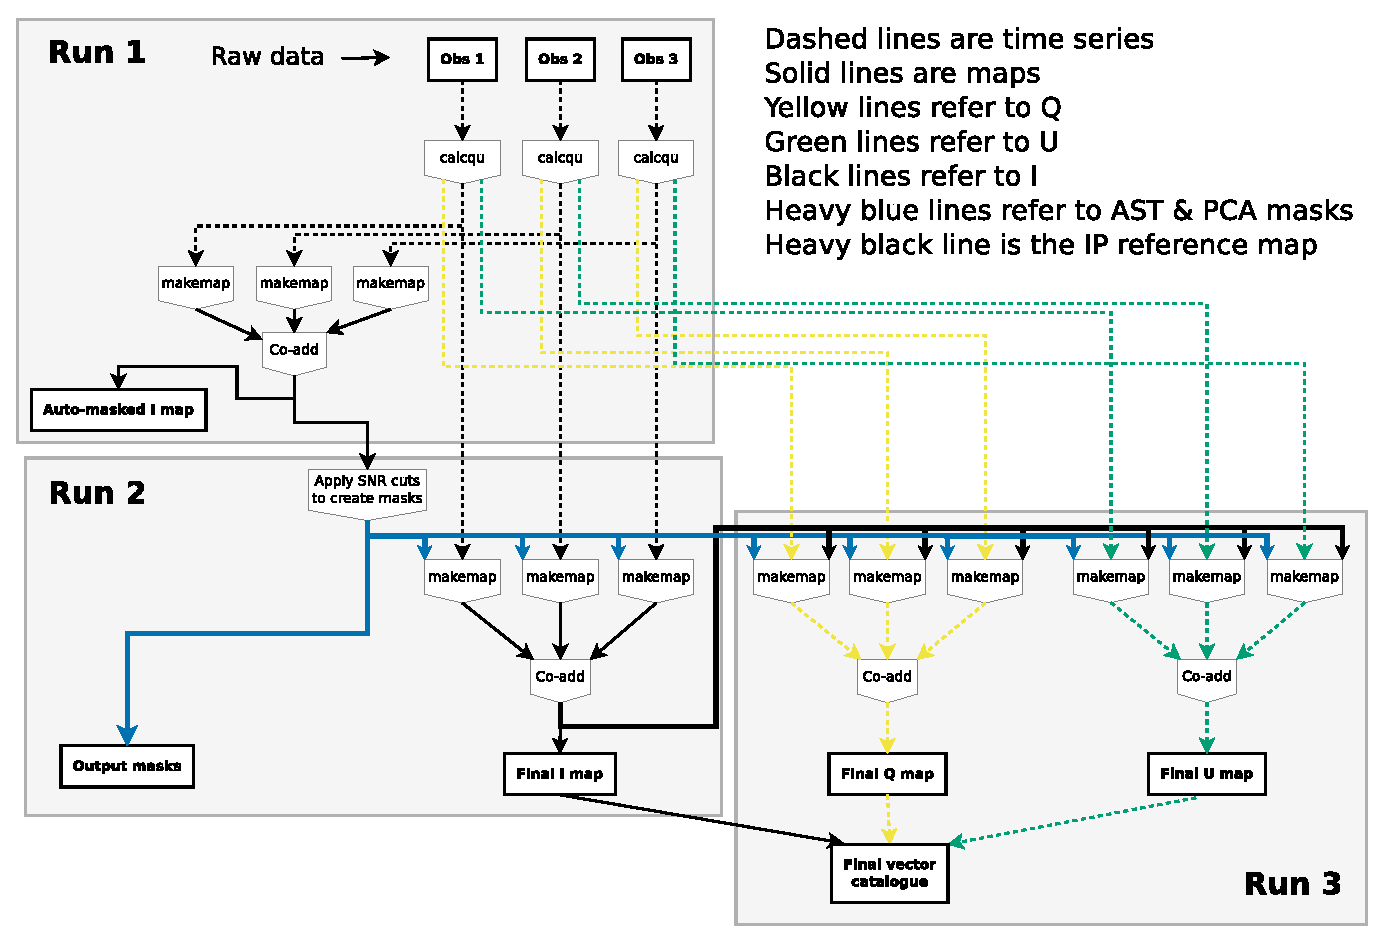
\includegraphics[width=0.85\linewidth,angle=90]{pol2map_flow}}{
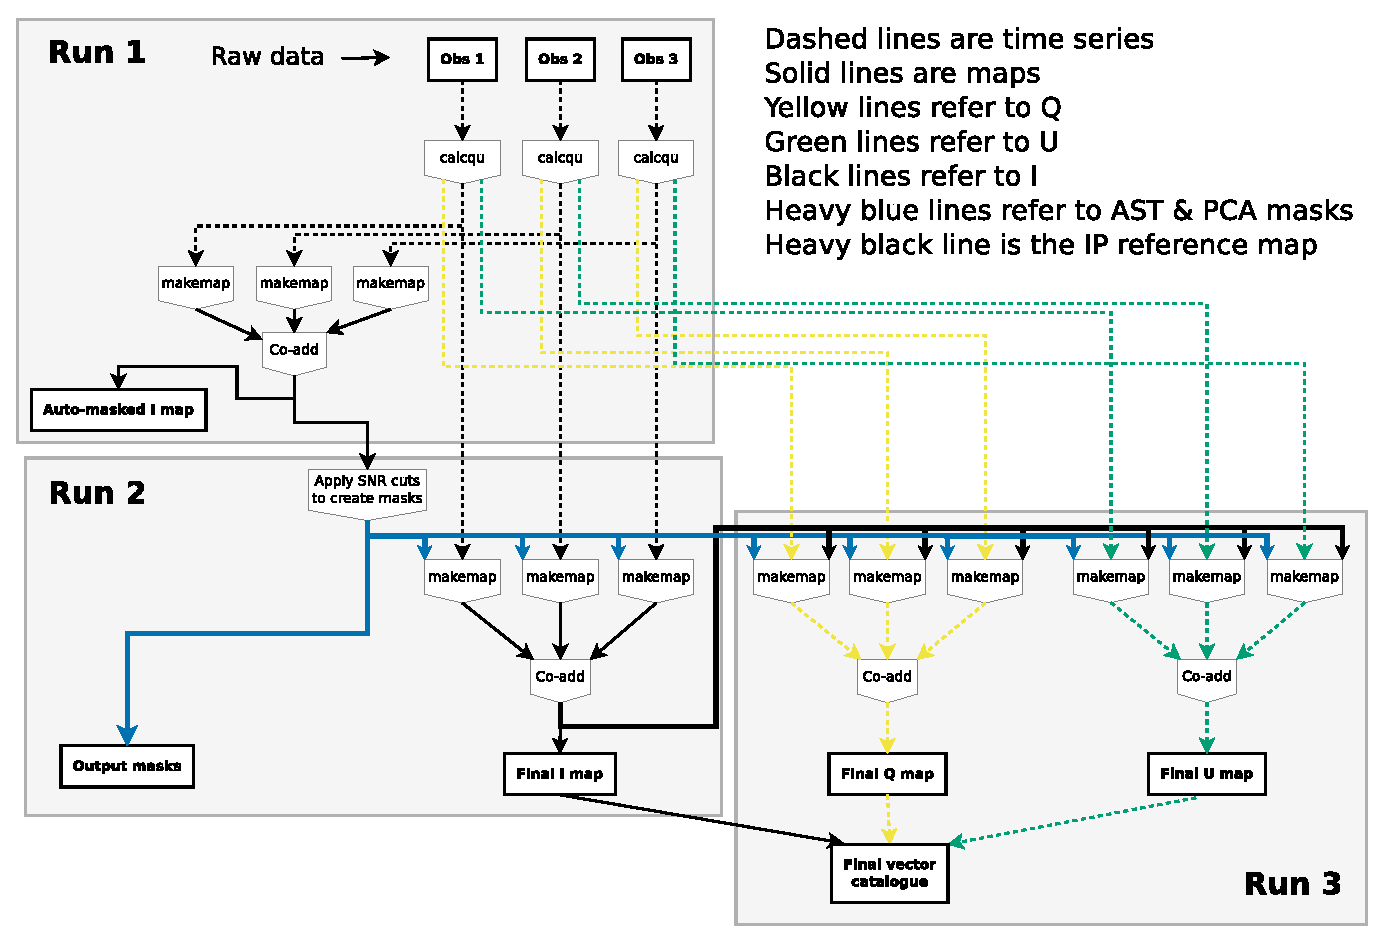
\includegraphics[width=1.0\linewidth]{pol2map_flow}}
\caption [POL-2 Data Flow]{ The data flow of the POL-2 data reduction
  method is presented. In this example, three POL-2 observations are
  reduced and combined in various stages and combination to produce I,
  Q and U maps and a vector catalogue.  }
\label{fig:pol2drflow}
\end{center}
\end{figure}


\subsection*{Step 1}

The initial step of the process (see Run~1 in Figure~\ref{fig:pol2drflow})
creates a preliminary co-added total intensity
(I) map from the raw data files for all observations provided to the
reduction routine (see \cref{Chapter}{sec:rundr}{}).


\subsubsection*{The process}
The analysed intensity values in the raw data time-streams are first
converted into Q, U and I time-streams using the
\xref{SMURF:\task{calcqu}}{sun258}{CALCQU} command (these are stored
for future use in the directory \texttt{qudata}, specified by the
\param{QUDIR} parameter in the example command below).

The \xref{SMURF:makemap}{sun258}{MAKEMAP} command is then used to
create a separate map from the I time-stream for each observation,
using SNR-based ``auto-masking'' to define the background regions that
are to be set to zero at the end of each iteration.

These maps are stored for future use in the directory \texttt{maps},
specified by the \param{MAPDIR} parameter. Each map has a name of the form:

\texttt{<UT$\_$DATE>$\_$<OBS$\_$NUM>$\_$<CHUNK$\_$NUM>$\_$imap.sdf}

where \texttt{<CHUNK$\_$NUM>} indicates the raw data file at the start
of the contiguous chunk of data used to create the map, and is usually
0003.  Each of these maps is compared to the specified reference map
(if any) to determine a pointing correction to be applied to the
observation in future. If no reference map is supplied, the I map
created from the first observation defines the expected source
position, and is compared with later maps to determine their pointing
corrections.

This step uses a PCA threshold of 50 (see Section~\ref{sec:pca} for more details).

\texttt{pca.pcathresh = -50}



\subsection*{Step 2}

In the second step of the process (see Run~2 in
Figure~\ref{fig:pol2drflow}) an improved I map is produced. These
improvements come from
\begin{enumerate}
\item applied relative pointing corrections
\item the use of an increased number of PCA components
  (\texttt{pca.pcathresh=-150})
\item using a single fixed mask for all observations. The mask is
  determined from the preliminary co-add I map and thus includes
  fainter structure than would be used if the mask was based on only
  one observation.
\end{enumerate}

\subsection*{Step 3}

In the third step of the reduction process (see Run~3 in
Figure~\ref{fig:pol2drflow}), both the Q and U maps are produced. The production
of the Q and U maps requires the Q and U time-series data (produced in
Step~1), the final I map (produced in Step~2) and the output masks (also
produced in Step~2). Once the Q and U maps are produced a final vector
catalogue is created.

\section{\xlabel{makemap}MAKEMAP}

The POL-2 data reduction builds upon the existing SCUBA-2 Dynamic
Iterative Map-Maker, hereafter just referred to as the map-maker. This
is the tool used to produce SCUBA-2 maps, and is invoked by the
\xref{SMURF:makemap}{sun258}{MAKEMAP} command. It performs some
pre-processing steps to clean the data, solves for multiple signal
components using an iterative algorithm, and bins the resulting
time-series data to produce a final science map.

In \poltwomap\ the map-maker is used in conjunction with
\xref{calcqu}{sun258}{CALCQU} (see
Section~\ref{sec:calcqu}) to produce maps of Q and U, as well as I.

\section{\xlabel{calcqu}CALCQU}
\label{sec:calcqu}

In addition to the POL-2 data reduction building on the
existing SCUBA-2 map-maker, \poltwomap\ also relies on the command
SMURF:CALQU.

This \xref{calcqu}{sun258}{CALCQU} tool creates time series holding Q and U values from a set of POL-2
time series holding raw data values. The supplied time-series data files are first
flat-fielded, cleaned and concatenated, before being used to create
the Q and U values. The Q and U time-series are down-sampled to 2Hz
(\emph{i.e.} they contain two Q or U samples per second), and are 
chosen to minimise the sum of the squared residuals between the measured 
raw data values and the expected values given by equation~\ref{eqn:idet}.


\section{\xlabel{pca}PCA}
\label{sec:pca}

One difference between the reduction of SCUBA-2 data and POL-2 data is the
method used to remove the sky background.  The sky background is usually
very large compared to the astronomical signal, and both are subject to
the same form of instrumental polarisation (IP - see Section~\ref{sec:ip}).
This
IP acting on the high sky background values causes high background values
in the Q and U maps. However, there is evidence that the IP is not
constant across the focal plane, resulting in spatial variations in the
background of the Q and U maps.

For non-POL-2 data, the background is removing using a simple common-mode
model, in which the mean of the bolometer values is found at each time
slice and is then removed from the individual bolometer values. This
ignores any spatial variations in the background and so fails to remove
the background properly in POL-2 Q and U maps.

To fix this, a second stage of background removal is used when processing
POL-2 data, following the initial common-mode removal. This second stage
is based upon a Principal Component Analysis (PCA) of the 1280
time-streams in each sub-array (the Q and U data are processed
separately). The PCA process identifies the strongest time-dependent
components that are present within multiple bolometers. These components
are assumed to represent the spatially varying background signal and are
removed, leaving just the astronomical signal. The number of components
to remove can be specified by the user, via a MAKEMAP configuration
parameter called `\xparam(PCA.PCATHRESH}{pca.pcathresh} although \poltwomap,
the reduction command for POL-2
data, provides suitable defaults for this parameter.

\begin{itemize}
\item first stage uses \param{pca.pcathresh} = -50
\item second stage uses \param{pca.pcathresh} = -150
\end{itemize}

On each MAKEMAP iteration, the PCA process removes the background (thus
reducing the noise in the map) but also removes some of the astronomical
signal. The amount of astronomical signal removed will be greater for
larger values of \texttt{pca.pcathresh}. However, this astronomical
signal is still present in the original time-series data and so can be
recovered if sufficient MAKEMAP iterations are performed. In other words,
using larger values of \param{pca.pcathresh} slows down the rate at
which astronomical signal is transferred from the time-series data to the
map, thus increasing the number of iterations required to recover the
full astronomical signal in the map.

Spatial variations in the sky background may also be present in non-POL-2
data, but at a lower level. For a discussion of why PCA is not routinely
run on non-polarimetric SCUBA-2 data, see \cref{Appendix}{app:pca}{}.



\section{\xlabel{masking}Masking}
A mask is a two-dimensional array which has the same shape and size as
the final map, and which is used to indicate where the source is
expected to fall within the map. `Bad' pixel values within a mask
indicate background pixels, and `good' pixel values indicate source
pixels. Masks are used for two main purposes:

\begin{enumerate}
\item To prevent the growth of gradients and other artificial large
  scale structures within the map.  For this purpose, the astronomical
  signal at all background pixels defined by the mask is forced to
  zero at the end of each iteration within MAKEMAP (except for the
  final iteration).
\item To prevent bright sources polluting the evaluation of the
  various noise models (PCA, COM, FLT) used within MAKEMAP. Source
  pixels are excluded from the calculation of these models.
\end{enumerate}


The \poltwomap\ script uses different masks for these two purposes - the
``AST'' mask and the ``PCA'' mask.  The PCA mask is in general less
extensive than the AST mask, with the source areas being restricted to
the brighter inner regions.  Each of these two masks can either be
generated automatically within \task{pol2map}, or be specified by a fixed
external NDF.



\section{\xlabel{tailoredDR}Tailoring a reduction}

\subsection*{Variances between POL-2 maps}

\param{MAPVAR} is a \poltwomap\ parameter that controls how the variances in the
coadded I, Q and U maps are formed.

If MAPVAR is set TRUE, the variances in the coadded I, Q and U maps
are formed from the spread of pixel data values between the individual
observation maps. If MAPVAR is FALSE (the default), the variances in
the coadded maps are formed by propagating the pixel variance values
created by MAKEMAP from the individual observation maps (these are
based on the spread of I, Q or U values that fall in each pixel).

Use MAPVAR=TRUE only if enough observations are available to make the
variances between them meaningful.A general lower limit on its value
is difficult to define, but is advised a minimum of 10 observations.


If a test of the effect of this option is required on a field for which
the I, Q and U maps from a set of individual observations are already
available, the following may be done:

\begin{terminalv}
% pol2map in=maps/\* iout=imapvar qout=qmapvar uout=umapvar mapvar=yes \
                   ipcor=no cat=cat_mapvar debias=yes
\end{terminalv}

assuming that the I, Q and U maps are in directory \texttt{maps}. The
variances in \texttt{imapvar.sdf}, \texttt{qmapvar.sdf} and
\texttt{umapvar.sdf} will be calculated using the new method, and
these variances will then be used to form the errors in the
\texttt{cat$\_$mapvar.FIT} catalogue.




\newpage
\chapter{\xlabel{pol2_dr}POL-2 Data Reduction - Running pol2map}
\label{sec:rundr}

The previous chapter, \cref{Chapter}{sec:dr}{POL-2 Data Reduction - The Theory}, described how pol2map produces I, Q and U maps from raw POL-2 data.
It showed that this reduction process - which uses pol2map - is a three-step process.

As with the other Python scripts in SMURF, you can get more information about the available
parameters by doing either:
\begin{terminalv}
% pol2map --help
\end{terminalv}
or
\begin{terminalv}
% smurfhelp pol2map
\end{terminalv}

\section{\xlabel{how-pol2map}How to use pol2map}

Before running pol2map directly, it is necessary need to ensure that the \starlink\ environment has been
initialised and the \smurf\ package started (see
\cref{Section}{sec:starinit}{Initialising Starlink} and
\cref{Section}{sec:packinit}{KAPPA and SMURF for data processing}).

This Chapter describes how to run the pol2map to first produce an initial I map
and then again to produce the final I, Q, U maps and vector catalogue. 

To run pol2map values need to be supplied for the 
following command-line parameters\footnote{Note the distinction between
``command-line parameters'' that are
supplied on the \texttt{pol2map} command line, and ``configuration parameters''
that are specified within a configuration file. Values for all
\emph{configuration} parameters are obtained using a single \emph{command-line}
parameter called \texttt{CONFIG}.} to produce the initial intensity image:



\begin{aligndesc}
\item[\texttt{IN}] A list of input NDFs containing raw POL-2 data.
There are many ways in which the list of files can be supplied,
as described in Section ``\xref{Specifying Groups of Objects}{sun95}{se_groups}''
in \xref{SUN/95}{sun95}{}. The easiest is to create a simple text
file containing the names of the raw data files -- one per line --- and
then supply the name of the text file, preceded by an up-caret character
(\,\texttt{\^{}}\,), as the value for parameter \texttt{IN}. Note, the names of
the raw data files can contain wildcards such as ``$*$'' and ``?''.

\item[\texttt{IOUT}]
The name of the NDF in which to store the the total intensity (I) map
incorporating all supplied observations. The supplied filename should either have a file type of
``\texttt{.sdf}'', or no file type at all (in which case \texttt{.sdf}
will be appended to the supplied value). Any existing file with the same
name will be overwritten.

\item[\texttt{QOUT}]
The output NDF in which to return the Q map including all supplied
observations. This will be in units of pW. Null (!) should be supplied if no Q
map is required.


\item[\texttt{UOUT}]
The output NDF in which to return the U map including all supplied
observations. This will be in units of pW. Null (!) should be supplied if no U
map is required.

\item[\texttt{MAPDIR}]
The name of a directory in which to put the Q, U and I maps made
from each individual observation supplied via ``IN'', before
coadding them. If
null is supplied, the new maps are placed in the same temporary
directory as all the other intermediate files and so will be
deleted when the script exists (unless parameter RETAIN is set
TRUE). Note, these maps are always in units of pW. Each one will
contain FITS headers specifying the pointing corrections needed
to align the map with the reference map. [!]


\item[\texttt{QUDIR}]
The name of a directory in which to put the Q, U and I time series
generated by SMURF:CALCQU, prior to generating maps from them. If
null (!) is supplied, they are placed in the same temporary directory
as all the other intermediate files and so will be deleted when the
script exists (unless parameter RETAIN is set TRUE). [!]
\end{aligndesc}

when the output intensity image is used to produce the final I, Q, U 
maps and vector catalogues additional command-line parameters are required:

\begin{aligndesc}

\item[\texttt{CAT}]
The output FITS vector catalogue. No catalogue is created if
null (!) is supplied. Note - currently, the Q, U  and PI values
in this catalogue will be in units of pW. [!]


\item[\texttt{MASK}]
Specifies the type of masking to be used within makemap (the
same type of masking is used to create all three maps - I, Q
and U).


\item[\texttt{MASKOUT1}]
If a non-null value is supplied for MASKOUT, it specifies the NDF
in which to store the AST mask created from the NDF specified by
parameter MASK. Only used if an NDF is supplied for parameter
MASK. [!]


\item[\texttt{MASKOUT2}]
If a non-null value is supplied for MASKOUT, it specifies the NDF
in which to store the PCA mask created from the NDF specified by
parameter MASK. Only used if an NDF is supplied for parameter
MASK. [!]


\item[\texttt{IPREF}]
The total intensity map to be used for IP correction. The map must
be in units of pW. If the same value is supplied for both IOUT
and IPREF, the output I map will be used for IP correction. [!]

\item[\texttt{DEBIAS}]
TRUE if a correction for statistical bias is to be made to
percentage polarization and polarized intensity in the output
vector catalogue specified by parameter CAT. [FALSE]



\end{aligndesc}



\section{\xlabel{how-step1}pol2map - producing the initial I map.}

As discussed in \cref{Chapter}{sec:dr}{POL-2 Data Reduction - The Theory} pol2map must first be run on the raw data to produce an initial I map.
In this first step:

\begin{terminalv}
% pol2map in=^myfiles.list iout=iauto qout=! uout=! mapdir=maps qudir=qudata
\end{terminalv}


Here, the file \texttt{myfiles.lis} contains a list of the raw data
files to be included in the map, and could (for instance) look like this:

\begin{terminalv}
% cat myfiles.lis
/jcmtdata/raw/scuba2/s8a/20160125/00043/*
/jcmtdata/raw/scuba2/s8b/20160125/00043/*
/jcmtdata/raw/scuba2/s8c/20160125/00043/*
/jcmtdata/raw/scuba2/s8d/20160125/00043/*
\end{terminalv}

This uses all available data for all four 850\,$\mu$m sub-arrays, for
observation 43 taken on 25th January 2016\footnote{The input files should all be
for a single waveband from one or more POL-2 observations --- do not mix files from
different wavebands and/or astronomical regions}. In addition, the data used in this example also
comes from observation 56 and 59 taken on January 11th 2016 (UT).

\begin{tip}

An up-caret ( $ \hat{} $ ) is required any time you are reading in a group
text file in Starlink. For the map-maker this includes the configuration
file (a group of configuration parameters) and the list of input files (a
group of NDFs \emph{e.g.} \texttt{in= $ \hat{} $ myfiles.lis}).

To check if the files are POL-2 files, run the \smurf\ command pol2check
\begin{terminalv}
%pol2check ^myfiles.list
\end{terminalv}
\end{tip}

Note that qout and uout are set to null values as no Q or U maps are required
to be produced during this initial step 1 reduction stage.

The following shows the output from running this initial pol2map command:

\begin{terminalv}
Logging to file pol2map.log
Calculating Q, U and I time streams from raw analysed intensity data...
   1/3: Processing 116 raw data files from observation 20160125_00043 ...
   2/3: Processing 116 raw data files from observation 20160112_00059 ...
   3/3: Processing 116 raw data files from observation 20160112_00056 ...

>>>>   Making I map from 20160125_00043_0003...

   Using pre-calculated pointing corrections of (0.0,0.0) arc-seconds
   Re-using previously created map 'maps/20160125_00043_0003_imap'

>>>>   Making I map from 20160112_00056_0003...

Storing pointing corrections of (1.889022181,2.8085505485) arc-seconds for future use

>>>>   Making I map from 20160112_00059_0003...

Storing pointing corrections of (2.13319187001,2.40199783004) arc-seconds for future use
Coadding I maps from all observations:
\end{terminalv}

The files and folders produced in this reduction are:


\begin{aligndesc}
\item[\texttt{pol2map.log}] 
A log file containing the output from the pol2map command.

\item[\texttt{qudata/}]
A folder containing the raw I, Q and U data for each sub array for each observation.

\item[\texttt{maps/}]
A folder containing the individual I maps from each separate observation \texttt{$\_$imap.sdf}.

\item[\texttt{CCDPACK.LOG}]
Output log containing information produced as pol2map relies on the CCDPACK command MAKEMOS
to combine POL-2 data.

\item[\texttt{iauto.sdf}]
Output total intensity file from an automatically generated astronomical mask.


\end{aligndesc}

The output I map, iauto.sdf, can be opened and viewed with GAIA.

\begin{figure}[t!]
\begin{center}
\includegraphics[width=0.8\linewidth]{sc22-gaia-view-iauto.png}
\label{fig:gaia-iauto}
\caption [I map in GAIA]{
  \small The I map, iauto.sdf, as viewed with GAIA.
}
\end{center}
\end{figure}

The maps folder contains the individual I maps from each separate observation:

\begin{terminalv}
20160112_00056_0003_imap.sdf  20160112_00059_0003_imap.sdf  20160125_00043_0003_imap.sdf
\end{terminalv}

and the qudata folder contains:

\begin{terminalv}
s8a20160112_00056_0003_IT.sdf  s8b20160112_00059_0003_IT.sdf  s8c20160125_00043_0003_IT.sdf
s8a20160112_00056_0003_QT.sdf  s8b20160112_00059_0003_QT.sdf  s8c20160125_00043_0003_QT.sdf
s8a20160112_00056_0003_UT.sdf  s8b20160112_00059_0003_UT.sdf  s8c20160125_00043_0003_UT.sdf
s8a20160112_00059_0003_IT.sdf  s8b20160125_00043_0003_IT.sdf  s8d20160112_00056_0003_IT.sdf
s8a20160112_00059_0003_QT.sdf  s8b20160125_00043_0003_QT.sdf  s8d20160112_00056_0003_QT.sdf
s8a20160112_00059_0003_UT.sdf  s8b20160125_00043_0003_UT.sdf  s8d20160112_00056_0003_UT.sdf
s8a20160125_00043_0003_IT.sdf  s8c20160112_00056_0003_IT.sdf  s8d20160112_00059_0003_IT.sdf
s8a20160125_00043_0003_QT.sdf  s8c20160112_00056_0003_QT.sdf  s8d20160112_00059_0003_QT.sdf
s8a20160125_00043_0003_UT.sdf  s8c20160112_00056_0003_UT.sdf  s8d20160112_00059_0003_UT.sdf
s8b20160112_00056_0003_IT.sdf  s8c20160112_00059_0003_IT.sdf  s8d20160125_00043_0003_IT.sdf
s8b20160112_00056_0003_QT.sdf  s8c20160112_00059_0003_QT.sdf  s8d20160125_00043_0003_QT.sdf
s8b20160112_00056_0003_UT.sdf  s8c20160112_00059_0003_UT.sdf  s8d20160125_00043_0003_UT.sdf
\end{terminalv}


\section{\xlabel{how-step23}pol2map - producing the I, Q, U maps and catalogue}


As discussed in \cref{Chapter}{sec:dr}{POL-2 Data Reduction - The Theory}, the I map output from the initial run of pol2map
is used to derive the final I, Q and U maps. If requested, a vector catalogue is also produced.

The second and third steps of the POL-2 data reduction process can be run via a single command:

\begin{terminalv}
% pol2map in=qudata/\* iout=iext qout=qext uout=uext mapdir=maps mask=iauto \
          maskout1=astmask maskout2=pcamask ipref=iext cat=mycat debias=yes
\end{terminalv}

The following shows the output from running this second pol2map command. First, pol2map produces
new I maps for each map, correcting the position using from the intensity map provided by mask 
(in this case iauto.sdf)and then coadds all the observations.

\begin{terminalv}
Logging to file pol2map.log
(existing file pol2map.log moved to pol2map.log.1)

Masking will be based on SNR values in 'iauto'.

>>>>   Making I map from 20160112_00056_0003...

   Using pre-calculated pointing corrections of (1.889022181,2.8085505485) arc-seconds

>>>>   Making I map from 20160125_00043_0003...

   Using pre-calculated pointing corrections of (0.0,0.0) arc-seconds

>>>>   Making I map from 20160112_00059_0003...

   Using pre-calculated pointing corrections of (2.13319187001,2.40199783004) arc-seconds
Coadding I maps from all observations:
\end{terminalv}

as pol2map continues, the Q and U maps are then produced, again with pointing corrections. This is followed by the creation of
the output vector catalogue:

\begin{terminalv}
>>>>   Making Q map from 20160112_00056_0003...

   Using pre-calculated pointing corrections of (1.889022181,2.8085505485) arc-seconds

>>>>   Making Q map from 20160125_00043_0003...

   Using pre-calculated pointing corrections of (0.0,0.0) arc-seconds

>>>>   Making Q map from 20160112_00059_0003...

   Using pre-calculated pointing corrections of (2.13319187001,2.40199783004) arc-seconds
Coadding Q maps from all observations:

>>>>   Making U map from 20160112_00056_0003...

   Using pre-calculated pointing corrections of (1.889022181,2.8085505485) arc-seconds

>>>>   Making U map from 20160125_00043_0003...

   Using pre-calculated pointing corrections of (0.0,0.0) arc-seconds

>>>>   Making U map from 20160112_00059_0003...

   Using pre-calculated pointing corrections of (2.13319187001,2.40199783004) arc-seconds
Coadding U maps from all observations:
Creating the output catalogue: 'mycat'...

45604 vectors written to the output catalogue.
\end{terminalv}


The output of this final run of pol2map is as follows:

\begin{aligndesc}
\item[\texttt{pol2map.log}] 
A log file containing the output from the pol2map command. Note previous log files
are moved to a new name such as \texttt{pol2map.log.1}.

\item[\texttt{astmask.sdf}]
The astronomical mask used in the creation of the final I, Q and U maps.

\item[\texttt{pcamask.sdf}]
The pca mask used in the creation of the final I, Q and U maps.

\item[\texttt{iext.sdf}]
The total intensity image, created using an external ast and pca mask.

\item[\texttt{qext.sdf}]
The intensity of the radiation linearly polarised in the direction parallel
 or perpendicular to the reference plane, created using an external ast and pca mask.

\item[\texttt{maps/}]
A folder containing the individual I, Q and U maps from each separate observation 
\texttt{$\_$Imap.sdf}, \texttt{$\_$Qmap.sdf} and \texttt{$\_$Umap.sdf}.

\item[\texttt{CCDPACK.LOG}]
Output log containing information produced as pol2map relies on the CCDPACK command MAKEMOS
to combine POL-2 data.

\item[\texttt{uext.sdf}]
The intensity of the radiation linearly polarised in the direction 45$^{\circ }$ to the
reference plane, created using an external ast and pca mask.

\item[\texttt{mycat.FIT}]
The output vector catalogue containing a range of values derived by pol2map for each pixel
contained within the I map.

\end{aligndesc}







\begin{figure}[t!]
\begin{center}
\includegraphics[width=0.46\linewidth]{sc22-gaia-view-iauto.png}
\includegraphics[width=0.46\linewidth]{sc22-gaia-view-iext.png}
\label{fig:gaia-iext}
\caption [Final I map in GAIA]{
  \small Left: I map, iauto, as produced by the automoask on the first pass of pol2map. Right: Final I map, iext, as viewed in GAIA.
}
\end{center}
\end{figure}


\begin{figure}[t!]
\begin{center}
\includegraphics[width=0.46\linewidth]{sc22-gaia-view-qext.png}
\includegraphics[width=0.46\linewidth]{sc22-gaia-view-uext.png}
\label{fig:gaia-qext-uext}
\caption [Q and U maps in GAIA]{
  \small Left: Q map, qext.sdf, Right: U map uext.sdf, as viewed with GAIA.
}
\end{center}
\end{figure}



The maps folder now contains individual Q and U maps alongside the existing I maps:

\begin{terminalv}
20160112_00056_0003_Imap.sdf  20160112_00059_0003_Imap.sdf  20160125_00043_0003_Imap.sdf
20160112_00056_0003_Qmap.sdf  20160112_00059_0003_Qmap.sdf  20160125_00043_0003_Qmap.sdf
20160112_00056_0003_Umap.sdf  20160112_00059_0003_Umap.sdf  20160125_00043_0003_Umap.sdf
20160112_00056_0003_imap.sdf  20160112_00059_0003_imap.sdf  20160125_00043_0003_imap.sdf
\end{terminalv}




\section{\xlabel{vector-cat}Output vectors from pol2map}



The output vector catalogue contains a range of values derived by pol2map for each pixel
contained within the I map. Values in the catalogue are expressed in units of Jy/beam.
The values are:

\begin{aligndesc}
\item[\texttt{X}] pixel coordinate
\item[\texttt{Y}] pixel coordinate
\item[\texttt{RA}] RA coordinate
\item[\texttt{Dec}] Dec coordinate
\item[\texttt{I}] Intensity
\item[\texttt{DI}] error in I
\item[\texttt{Q}] stokes Q parameter
\item[\texttt{DQ}] error in Q
\item[\texttt{U}] stokes U parameter
\item[\texttt{DU}] error in U
\item[\texttt{P}] Percentage Polarization
\item[\texttt{DP}] error in P
\item[\texttt{ANG}] angle of polarization
\item[\texttt{DANG}] error in ANG
\item[\texttt{PI}] Polarized Intensity
\item[\texttt{DPI}] error in PI
\end{aligndesc}




\section{\xlabel{tweaking}Tweaking pol2map}
\label{sec:pol2map-tweaks}

Inevitably, as with unpolarised SCUBA-2 data reduction, it will probably be necessary for a user to
tweak the pol2map reduction for specific situations.

The pixel size of the final map produced is controlled by the pixsize
parameter in the the \smurf\ pol2map command:

\begin{terminalv}
% pol2map pixsize=12
\end{terminalv}









\newpage
\chapter{\xlabel{pol2_image}POL-2 Image Display}
\label{sec:display}

\section{\xlabel{gaia}GAIA}

The \starlink\ package \gaia\ can be used to inspect the results of the data reduction. 
To plot the output vector catalogue onto the final non-polarized intensity map
first open up the I map in gaia:

\begin{terminalv}
% gaia iext.sdf
\end{terminalv}


Then In the main Gaia window, select the drop-down menu option Image Analysis / 
Polarimetry toolbox…. This should launch a new toolbox window entitled 
GAIA: Polarimetry. From this window, use the drop-down menu option 
File / Open to load the file mycat.FIT. This should then populate the lower part of the 
window with the contents of this polarimetry catalogue file. 
Each of the vectors in this file will be automatically overlaid on the main image window 
(see figure \ref{fig:gaia-plot-vectors1}).

\begin{figure}[t!]
\begin{center}
\includegraphics[width=0.46\linewidth]{sc22-gaia-plot-vectors-1.png}
\includegraphics[width=0.46\linewidth]{sc22-gaia-plot-vectors-3.png}
\label{fig:gaia-plot-vectors1}
\caption [Over Plotting Vectors in GAIA]{
  \small Left: Opening up the polarimetry tool box in GAIA. Right: The initial POL-2 
vectors overplotted in GAIA.
}
\end{center}
\end{figure}

In order to filter the number of overlaid vectors down to a more useful number and size,
various options in the GAIA: Polarimetry window can be used. First, select the Rendering
tab on the left hand side. This will reveal a panel that will indicate which quantities 
are currently being used for the vector overlays. In this case, the Vector length is taken 
from the P column of the table, and the Vector angles are taken from the ANG column.

Currently the figure has too many vectors to be scientifically meaningful. To filter 
out most of the extraneous vectors, click on the Selecting tab, and set the Expression 
field to be the following:

\begin{terminalv}
$I/$DI>10
\end{terminalv}

\emph{Ensure you press return after entering in the above expression}.

The above expression selects the data points in the polarimetry table which have an 
associated non-polarized intensity (column I) more than 10 times greater than the 
associated error value for that intensity (column DI). To remove all of the other 
extraneous overlaid vectors, click on the Invert selection button in the GAIA: Polarimetry 
window, and then use the drop-down menu option Edit / Cut. This should leave just a 
small number of vectors clustering around the target object. 

\begin{figure}[t!]
\begin{center}
\includegraphics[width=0.46\linewidth]{sc22-gaia-plot-vectors-4.png}
\includegraphics[width=0.46\linewidth]{sc22-gaia-plot-vectors-6.png}
\label{fig:gaia-plot-vectors2}
\caption [Selecting Vectors in GAIA]{
  \small Left: specifying vectors to display via the expression \$I/\$DI$>$10. This will only plot
vectors with an 850 micron intensity signal-to-noise ratio grater than 10 in GAIA. To ensure this is selected
ensure you press the carriage return after entering the expression. 
}
\end{center}
\end{figure}

Zooming in on the central region of the map, it can already be seen that the level of vector ordering 
(and hence polarization) is quite low (see figure \ref{fig:gaia-plot-vectors3}). If needed it is 
possible to change the scaling by selecting the Rendering tab in the GAIA: Polarimetry 
window, and increasing the vector scale.


\begin{figure}[t!]
\begin{center}
\includegraphics[width=0.44\linewidth]{sc22-gaia-plot-vectors-5.png}
\includegraphics[width=0.52\linewidth]{sc22-gaia-plot-vectors-7.png}
\label{fig:gaia-plot-vectors3}
\caption [Over Plotting Vectors in GAIA]{
  \small Left: Selected vectors are marked in blue in this example, Right: after removal of selected
vectors all that remains are the vectors on the regions where \$I/\$DI$>$10. 
}
\end{center}
\end{figure}


\section{\xlabel{kappa}kappa}



\newpage
\chapter{\xlabel{pol2_advanced}POL-2 -- Advanced Data Reduction}
\label{sec:advanced}


The \poltwomap\ tool for reducing POL-2 data was released to the science
community for the start of 17B observing. As with all newly
commissioned instrumentation the ``ideal'' reduction has yet to be
finalised. This advanced section of the POL-2 data reduction
documentation aims to provide you with tools for
expanding and examining the POL-2 reduction process further and in
more detail.

For further ideas, see \cref{Section}{sec:tailoredDR}{Tailoring a reduction}.

\section{\xlabel{addingdata}Adding new observations}

This section describes the six-step process of combining data for one
or more new POL-2 observations into existing I, Q and U maps and vector
catalogue created by an earlier run of \task{pol2map}.

\begin{enumerate}

\item Create a text file listing all the existing auto-masked I maps
  for individual observations stored in the directory specified by
  Parameter \param{MAPDIR}, and then add in the raw data files for the new
  observations. The auto-masked I maps have names that end in
  \file{$\_$imap.sdf}.

\begin{terminalv}
% ls maps/*imap.sdf > infiles.list
% ls rawdata/*.sdf  >> infiles.list
\end{terminalv}


\item Create a new auto-masked, co-added I map including the new
  observation. The \xref{calcqu}{sun258}{CALCQU} and \makemap\ commands
  will be run on the new
  data and the resulting maps combined with the existing maps derived
  from the older observations to create the new map.

\begin{terminalv}
% pol2map in=^infiles iout=iauto_new qout=! uout=! mapdir=maps \
     qudir=qudata
\end{terminalv}


\item A decision needs to be taken whether to re-create all the
  externally masked maps using external masks defined by the new
  auto-masked map. This will be the case if the auto-masked map has
  been changed significantly by the addition of the new
  observation. To do this, it is necessary to compare the old and new
  masks. The old masks should have been created earlier using the
  \param{MASKOUT1} and \param{MASKOUT2} parameters (see Step~3 in
  \cref{Section}{sec:dr}{POL-2 Data Reduction -- The Theory}). To
  create the new masks that would be generated from the new
  auto-masked map, use this command.

\begin{terminalv}
% pol2map  in=^infiles iout=! qout=! uout=! mapdir=maps mask=iauto_new \
     maskout1=astmask_new  maskout2=pcamask_new
\end{terminalv}

\item Decide if the addition of the new data has changed the masks
  significantly. This involves comparing \file{astmask.sdf} and
  \file{astmask$\_$new.sdf} (and also \file{pcamask.sdf} and
  \file{pcamask$\_$new.sdf}).


\item If the mask has changed significantly and all observations need
  to be reprocessed using the new mask, remove the existing
  externally-masked maps so that they will be re-created by the next
  invocation of \task{pol2map}.  Note -- this will increase the length of time
  taken by Step~6 enormously.

  Ensure the new auto-masked co-add is used in place of the old one to
  define any new masks needed in future.

\begin{terminalv}
% rm mapdir/*Qmap.sdf mapdir/*Umap.sdf mapdir/*Imap.sdf
% mv iauto.sdf iauto_old.sdf
% mv iauto_new.sdf iauto.sdf
\end{terminalv}

\item Re-create the necessary externally masked maps and co-adds, and
  then create the new vector catalogue.

\begin{terminalv}
% pol2map in=qudata/\* iout=iext_new qout=! uout=! mapdir=maps \
     mask=iauto
% pol2map in=qudata/\* iout=! qout=qext_new uout=uext_new mapdir=maps \
     mask=iauto ipref=iext_new cat=mycat_new debias=yes
\end{terminalv}
\end{enumerate}


\section{\xlabel{pixelsize}Experimenting with pixel sizes}

Currently,the default map pixel size is 4\si{\arcsecond} at both
450 and \SI{450}{\micro\metre}. The pixel size is controlled by the
\param{PIXSIZE} parameter in the \smurf\ \poltwomap\ command:

\begin{terminalv}
% pol2map pixsize=12
\end{terminalv}


The following four-step example shows how to investigate the impact of
changing pixel size.  In this example, we compare 12\si{\arcsecond}
pixels and 7\si{\arcsecond} pixels.

\begin{enumerate}
\item Begin with an auto-masked total-intensity map from the raw
  data. For instance:

\begin{terminalv}
% pol2map in=^myfiles.list iout=iauto12 pixsize=12 qout=! uout=! \
     mapdir=maps12 qudir=qudata
\end{terminalv}


\item Create AST and PCA masks with 12\si{\arcsecond} pixels from the
  \file{iauto12.sdf} file.


\begin{terminalv}
% pol2map in=qudata/\* iout=! qout=! uout=! mapdir=maps12 mask=iauto12 \
     maskout1=astmask12 maskout2=pcamask12
\end{terminalv}

\item Create masks with 7\si{\arcsecond} pixels by resampling the
  12\si{\arcsecond} masks created at Step~2. This is done using the
  \Kappa\ \xref{\task{sqorst}}{sun95}{SQORST} command:

\begin{terminalv}
% sqorst  mode=pixelscale pixscale=\'7,7,7E-05\' in=astmask12 out=astmask7
% sqorst  mode=pixelscale pixscale=\'7,7,7E-05\' in=pcamask12 out=pcamask7
\end{terminalv}

\item Create the 7\si{\arcsecond} externally masked I, Q and U maps
  using the above 7\si{\arcsecond} masks (note the \texttt{mask}
  parameter value is enclosed in single \emph{and} double quotes).

\begin{terminalv}
% pol2map in=qudata/\* iout=iext7 qout=qext7 uout=uext7 masktype=mask \
                  mask="'astmask7,pcamask7'" mapdir=maps7 ipref=iext7  \
                  cat=cat7 debias=yes
\end{terminalv}
\end{enumerate}

\begin{tip}
  Using larger pixels usually produces slower convergence, so the
  above process will take longer than usual -- be patient!

  Using larger pixels can sometimes encourage smooth blobs and other
  artificial features to appear in the map. The \file{iauto12.sdf} file
  should be examined to check that it does not have such artificial
  features.

  Check the masks (\file{astmask12.sdf} and \file{pcamask12.sdf}) to make sure they
  look reasonable.

  It is usually advisable to leave \param{PIXSIZE} at its default value
  and instead use the \param{BINSIZE} parameter to control the bin size in
  the vector catalogue---see \cref{Section}{sec:pol2map-pixelsize}{Changing pixel size in pol2map}).
\end{tip}

\section{\xlabel{IPerror}Investigating systematic error in IP}


The error on the IP is reported to be of the order of 0.5\%.  It is
possible to investigate the effects of the systematic error in IP by
creating maps using the upper and lower limits on the IP value. The
\task{makemap} configuration parameter called \xparam{IPOFFSET}{ipoffset}
can be used to do such an
investigation. To use it, run \task{pol2map} twice as follows:

\begin{terminalv}
% pol2map config="ipoffset=-0.25"
% pol2map config="ipoffset=0.25"
\end{terminalv}

to produce maps using the upper and lower IP limits (a range of
0.5\%). If \task{pol2map} has already been run on POL-2 data then a file will
already exist that was created using the mean IP (the mean IP is used
if \param{ipoffset} is omitted from the configuration value, or the
configuration parameter itself is omitted).

%\section{\xlabel{simulations}Simulated data}


\section{\label{sec:wcscopy}Adding WCS information back into a vector catalogue}
Vector catalogues produced by \task{pol2map} contain information about World Coordinate
Systems (WCS) in two different forms:

\begin{enumerate}
\item The catalogue contains ``RA'' and ``Dec'' columns that hold the sky position
(FK5, J2000) of each vector, in radians.
\item The catalogue header contains a Starlink ``WCS FrameSet'' which defines
(amongst other things) the projection from pixel coordinates within the I, Q and
U mosaics, to RA and Dec. This FrameSet is used by Starlink software, together
with the pixels coordinates stored in the ``X'' and ``Y'' columns, to determine
the RA and Dec of each vector. The WCS FrameSet also defines the polarimetric
reference direction used by the Q, U and ANG values. See
``\xref{Using World Co-ordinate Systems}{sun95}{se_wcsuse}''
within \xref{SUN/95}{sun95}{} (the \KAPPA\ manual) for more information on
the ways in which Starlink software handles WCS information.
\end{enumerate}

Starlink software such as \polpack, \Kappa\ and \gaia\ rely on the WCS
FrameSet for all WCS-related operations (drawing annotated axes, aligning
data sets, \emph{etc}). Thus problems are likely if the WCS FrameSet is
removed from the vector catalogue. This could happen for instance if you
use inappropriate software to process an existing catalogue, creating a
new output catalogue -- the WCS FrameSet may not be copied to the output
catalogue, causing subsequent WCS-related operations to fail. It is safe
to use \POLPACK, \KAPPA, \GAIA\ and \xref{\textsc{Cursa}}{sun190}{}) as
all these packages copy the WCS FrameSet to any new output catalogues.
Unfortunately, the popular \topcat\ catalogue browser (see
\url{http://www.starlink.ac.uk/topcat/}) and the STILTS package
(\url{http://www.starlink.ac.uk/stilts/}) upon which it is based, do
\emph{not} copy the WCS FrameSet to any output catalogues.

For this reason, \POLPACK\ contains a command that can be used to copy the
WCS FrameSet from one catalogue to another.  Say for instance you create
catalogue \file{mycat.FIT} using \task{pol2map}, and then use \textsc{Topcat} to remove
low signal-to-noise vectors, saving the results to a new catalogue called
\file{selcat.FIT}. The WCS FrameSet will be missing from \file{selcat.FIT},
and so we need to copy it back again from the original catalogue \file{mycat.FIT}.
To do this we use the ``\xref{polwcscopy}{sun223}{POLWCSCOPY}'' command:

\begin{terminalv}
% polwcscopy in=selcat ref=mycat out=selcat2
\end{terminalv}

This creates a third catalogue \file{selcat2.FIT}, which is a copy of
\file{selcat.FIT} but with WCS inherited from \file{mycat.FIT}.







\newpage
\begin{thebibliography}{}
\addcontentsline{toc}{section}{References}



\bibitem{archibald}
Archibald,~E.~N., et~al, 2002, \htmladdnormallink{\textit{On the atmospheric limitations
of ground-based submillimetre astronomy using array receivers}}{http://dx.doi.org/10.1046/j.1365-8711.2002.05582.x}, MNRAS, 336, 1-13
(DOI:10.1046/j.1365-8711.2002.05582.x)

\bibitem{Bastien2011}
Bastien,~P.,et~al., 2011, \htmladdnormallink{\textit{POL-2: The SCUBA-2 Polarimeter}}{http://aspbooks.org/custom/publications/paper/449-0068.html} ASP, 449, 68B

\bibitem{fellwalker}
Berry~D.~S.,  2015,
\htmladdnormallink{\textit{FellWalker - a Clump Identification Algorithm}}
{http://dx.doi.org/10.1016/j.ascom.2014.11.004},
Ast. \& Comp., 10, 22-31 (DOI:10.1016/j.ascom.2014.11.004)

\bibitem{polpack}
Berry~D.~S, Gledhill~T.~M, 2015, \textit{POLPACK -- An Imaging Polarimetry Reduction Package},
\xref{Starlink User Note 223}{sun223}{}

\bibitem{oracdr}
Cavanagh~B., Jenness~T., Economou~F., Currie~M.~J., 2008,
\htmladdnormallink{\textit{The ORAC-DR data reduction
pipeline}}{http://dx.doi.org/10.1002/asna.200710944}, Astron. Nactr., 329, 295
(DOI:10.1002/asna.200710944)

\bibitem{smurf}
Chapin~E.~L., et~al., 2013, \textit{SMURF -- Sub-Millimetre User Reduction
Facility}, \xref{Starlink User Note 258}{sun258}{}

\bibitem{mapmaker}
Chapin~E.~L., et~al., 2013,
\htmladdnormallink{\textit{SCUBA-2: iterative map-making with the
Sub-Millimetre User Reduction Facility}}{http://dx.doi.org/10.1093/mnras/stt052},
MNRAS, 430, 2545 (DOI:10.1093/mnras/stt052)

\bibitem{ssds}
Currie~M.~J., Wallace~P.~T., Warren-Smith~R.~F., 1989,
\textit{Starlink Standard Data Structures}, \xref{Starlink General
Paper 38.2}{sgp38}{}

\bibitem{kappa}
Currie~M.~J., Berry~D.~S, 2013, \textit{KAPPA -- Kernel Application Package},
\xref{Starlink User Note 95}{sun95}{}

\bibitem{dempsey12}
Dempsey~J.~T. et al., 2013, \htmladdnormallink{\textit{SCUBA-2: on-sky calibration using
submillimetre standard sources}}{http://dx.doi.org/10.1093/mnras/stt090},
MNRAS, 430, 2534 (DOI:10.1093/mnras/stt090)

\bibitem{dempsey-spie}
Dempsey~J.~T., Friberg~P., Jenness~T., Bintley~D., Holland~W.~S., 2010
\htmladdnormallink{\textit{Extinction correction and on-sky calibration of
SCUBA-2}}{http://dx.doi.org/10.1117/12.856476},
Proc.\ SPIE, 7741 (DOI:10.1117/12.856476)

\bibitem{gaia}
Draper~P.~W., Gray~N., Berry~D.~S., Taylor~M., 2012,
\textit{GAIA -- Graphical Astronomy and Image Analysis Tool},
\xref{Starlink User Note 214}{sun214}{}

\bibitem{Friberg}
Friberg,~P., et~al, 2016, \htmladdnormallink{\textit{POL-2: a polarimeter
for the James-Clerk-Maxwell telescope}}{http://proceedings.spiedigitallibrary.org/proceeding.aspx?articleid=2536885},
SPIE, Volume 9914, id. 991403
(DOI: 10.1117/12.2231943)

\bibitem{picard}
Gibb~A.~G., Jenness~T., Economou~F., 2012, \textit{PICARD --- a
PIpeline for Combining and Analyzing Reduced Data}
\xref{Starlink User Note 265}{sun265}{}

\bibitem{s2main}
Holland, W. S., et~al, 2013, \htmladdnormallink{\textit{SCUBA-2: The
10,000 pixel bolometer camera on the James Clerk Maxwell Telescope}}
{http://dx.doi.org/10.1093/mnras/sts612}, MNRAS, 430, 2513
(DOI:10.1093/mnras/sts612)

\bibitem{flux1}
Jenness~T., et~al, 2002, \htmladdnormallink{\textit{Towards the automated
reduction and calibration of SCUBA data from the James Clerk Maxwell
Telescope}}{http://dx.doi.org/10.1046/j.1365-8711.2002.05604.x},
MNRAS, 336, 14-21 (DOI:10.1046/j.1365-8711.2002.05604.x)

\bibitem{ndf}
Jenness~T., et~al, 2014,
\htmladdnormallink{\textit{Learning from 25 years of the extensible
N-Dimensional Data Format}} {http://dx.doi.org/10.1016/j.ascom.2014.11.001},
Ast. \& Comp., 12, 146, (DOI:10.1016/j.ascom.2014.11.001)

\bibitem{Savini}
Savini, G., et~al. 2009, \htmladdnormallink{\textit{Recovering the frequency
dependent modulation function of the achromatic half-wave plate for POL-2:
the SCUBA-2 polarimeter}} {https://doi.org/10.1364/AO.48.002006},
Applied Optics, 48, 2006
(DOI: 10.1364/AO.48.002006)

\bibitem{sc2ana005}
Scott~D., Van Engelen~A., 2005, \htmladdnormallink{\textit{Scan Mode Strategies for
SCUBA-2}}{http://docs.eao.hawaii.edu/JCMT/SC2/ANA/S210/005/sc2_ana_s210_005.ps},
SCUBA-2 Data Reduction document SC2/ANA/S210/005

\end{thebibliography}

\newpage
\appendix
\chapter{\xlabel{pca_scuba2}PCA on SCUBA-2 data}
\label{app:pca}

This document has outlined the process of reducing POL-2 data and its
reliance on PCA during the makemap process. There are two main reasons 
why running make-map with PCA is not the default method for all data observed
using SCUBA-2:

\begin{enumerate}
\item It is time-consuming to run;
\item It produces similar results to running the default makemap with an increasing the filter size.
\end{enumerate}

All the relevant tools are still provided however, and so interested users
may wish to try using this method and to compare the results.




\end{document}

